\documentclass[a4paper]{article}
\usepackage{fancyhdr}
\usepackage[includeheadfoot,left=1in, right=0.5in, top=0.5in, bottom=0.5in]{geometry}
\usepackage{lastpage}
\usepackage{extramarks}
\usepackage[usenames,dvipsnames]{color}
\usepackage{graphicx}
\usepackage{listings}
\usepackage{courier}
\usepackage{tikz}
\usepackage{color}
\usepackage{float}
\usepackage{url}
\usepackage{subfigure}
\usepackage{varwidth}
\usepackage{caption}
\usepackage{multirow}
\usepackage[pdfborder={0 0 0}]{hyperref}
\usepackage[compact,small]{titlesec}
\usepackage{microtype}
\usepackage{verbatim}
\usepackage{booktabs}
\usepackage{indentfirst}
\usepackage{enumitem}
\usepackage{pdfpages}
\usepackage{epstopdf}

\captionsetup[sub]{labelsep=newline}

% line spacing
\linespread{2.0}

% bold item
\let\origitem\item
\renewcommand{\item}{\normalfont\origitem}
\newcommand{\bolditem}{\small\bfseries\origitem}

% tilde
%\newcommand{\small_tilde}{\raise.17ex\hbox{$\scriptstyle\sim$}}

% indent item
\newcommand{\indentitem}{\setlength\itemindent{24pt}}

% perfect tilde
\newcommand{\tildep}{\raise.17ex\hbox{$\scriptstyle\sim$}}

\parskip = 0.5\baselineskip
\setlength{\belowcaptionskip}{-\baselineskip}

\captionsetup{font=scriptsize}
\captionsetup{labelfont=bf}

\pagestyle{fancy}
\rhead{\fancyplain{}{\rightmark }}
\lhead{\fancyplain{}{\leftmark }}
\rfoot{Page\ \thepage\ of \protect\pageref{LastPage}}
\cfoot{}
\renewcommand\headrulewidth{0.4pt}
\renewcommand\footrulewidth{0.4pt}

% make verbatim text small
\makeatletter
\g@addto@macro\@verbatim\small
\makeatother

%\setlength\parindent{0pt} % Removes all indentation from paragraphs
\setlength\parindent{24pt}

\definecolor{sh_comment}{rgb}{0.12, 0.38, 0.18 } %adjusted, in Eclipse: {0.25, 0.42, 0.30 } = #3F6A4D
\definecolor{sh_keyword}{rgb}{0.37, 0.08, 0.25}  % #5F1441
\definecolor{sh_string}{rgb}{0.06, 0.10, 0.98} % #101AF9

%\sectionfont{\centering}
\lstset{
    language=vhdl,
    xleftmargin=.25in,
    xrightmargin=.25in,
    numbers=left,
    numberstyle=\tiny,
    frame=tb,
    showstringspaces=false,
    captionpos=b,
    stringstyle=\color{sh_string},
    keywordstyle = \color{sh_keyword}\bfseries,
    commentstyle=\color{sh_comment}\itshape,
    basicstyle=\small\sffamily,
    %numbersep=-5pt,
    belowskip=\baselineskip,
    aboveskip=\baselineskip
}
\usepackage{authblk}

\title{
    \vspace{2in}
    \textbf{Cluster Headaches and Other Stories \\}
    \vspace{2in}
}

\author{Eric Carver}

\affil{carverer@mail.uc.edu}
    \vspace{10pt}

\affil{(513) 207-6501}
    \vspace{2.0in}

\titleformat*{\section}{\large\normalfont}

\begin{document}

%\includepdf{}
\maketitle
\thispagestyle{empty}
\newpage
\thispagestyle{empty}
\parskip = 0.2\baselineskip
\newpage
\thispagestyle{empty}
\section*{\textbf{Abstract}}
\newpage
\thispagestyle{empty}
\section*{\textbf{Acknowledgements}}
\newpage
\thispagestyle{empty}
\tableofcontents
\newpage
\thispagestyle{empty}
\listoffigures
\listoftables
\parskip = 0.5\baselineskip
\newpage

\section{\textbf{Introduction}}
\label{introduction}

\subsection{\textbf{Research Statement}}

This research will make the 

\subsection{\textbf{Thesis Overview}}

The remainder of this thesis is organized as follows.

Chapter \ref{background} provides background information on Parallel Discrete
Event Simulation (PDES), Infiniband\texttrademark, and small form factor
computers, including the ODROID platform used in this research.

Chapter \ref{latency_reduction} presents our strategy for attacking the network
latency problem in our Beowulf cluster. It focuses on two low-cost solutions:
software RDMA over Converged Ethernet (RoCE) and polling network drivers.

Chapter \ref{cluster} describes the hardware and software implementation of the
ODROID-XU cluster constructed as part of these experiments and details the
benchmarks and simulations used to test its performance.

Chapter \ref{results} provides the results of these tests and attempts to relate
the cluster's performance to its cost. The results of a similar set of tests on
a traditional cluster are provided for comparison.

Chapter \ref{conclusions} contextualizes the results of this research and
suggests ways to continue this work.

\newpage
\section{\textbf{Background}}
\label{background}

\subsection{\textbf{Parallel Discrete Event Simulation}}

\subsection{\textbf{Infiniband and RoCE}}

\href{www.infinibandta.org}{InfiniBand}\texttrademark (IB) was introduced in
1999 to meet the new demand of data-intensive applications in high-end computing
environments \cite{InfiniBandTABase-07}. Its characteristic high bandwidth and
low latency make it a popular interconnect technology for computing solutions
intended for fine-grained parallel simulation. For high-end Beowulf Clusters,
message latency as low as one microsecond is provided through the two-pronged
approach of using InfiniBand networking hardware and the lightweight IB
transport layer. However, the high cost and lack of inter-fabric compatibility
of such hardware have driven the development of solutions based on the
ubiquitous Ethernet link layer \cite{roce-announce}.

Although IB is a full first-order interconnect solution, its transport layer is
particularly attractive to researchers who desire affordable high performance
computing. It specifies four transport types: Reliable Connection (RC), Reliable
Datagram (RD), Unreliable Connection (UC), and Unreliable Datagram (UD)
\cite{InfiniBandTABase-07}. All four types support channel messaging semantics,
wherein messages are passed using send and receive calls
\cite{InfiniBandTABase-07}. The RC and UC types support memory semantics, also
known as Remote Direct Memory Access (RDMA). This approach allows an initiator
computing node to access the memory of a remote process directly, without any
significant effort on the part of the remote node \cite{sur-11}.

RDMA over Converged Ethernet (RoCE), also known as Infiniband over Ethernet
(IBoE), is an attempt to provide the reliable, low-latency InfiniBand transport
services over a converged Ethernet fabric already present in most data centers
\cite{InfiniBandTARoCE-10}, \cite{roce-announce}. This enables properly
configured networks to carry IB traffic without investing in entirely new
physical hardware. Message latency can be under 2 microseconds when used in a
lossless 40 Gigabit Ethernet network \cite{vienne-12}. RoCE has found a niche in
commercial data centers, especially those that support financial operations such
as high frequency trading. Unfortunately, specialized network adaptors are still
required to take advantage of its features. Additionally, these solutions
generally require switches that support Data Center Bridging (DCB)
\cite{InfiniBandTARoCE-10}. This creates an opportunity for a solution that can
work with existing lossy Ethernet networks.

%% TODO: Discuss iWARP

System Fabric Works, Inc., has created a pure software implementation of RoCE
called \href{http://www.systemfabricworks.com/downloads/roce}{rxe}. rxe is a
Linux driver that implements the full IB transport over any Ethernet adaptor
\cite{pearson-10}. Message latency can be as low as 10
microseconds\cite{pearson-10}. The
\href{http://support.systemfabricworks.com/downloads/rxe/}{most recent relase of
the driver} is in the from of patches for the mainline Linux kernel. We chose
to port this implementation to the ODROID platform for our studies in low-cost
Beowulf Clusters.


\subsection{\textbf{ODROID Platform}}

\subsubsection{\textbf{ODROID-U2}}

\subsubsection{\textbf{ODROID-XU}}

\subsection{\textbf{Related Work}}

%% ERIC: do we know of any related work?  even publications talking about
%% IBoE/RoCE performance on the x86 platform would be worth reviewing.

Although performance profiling of hardware IB and RoCE is extensive
\cite{subamaroni-09}, \cite{vienne-12}, studies on software RoCE are
rare. Robert J. Lancaster \cite{lancaster-10} experimented with the rxe
driver. He found that rxe message latency ranged from 14\% to 81\% lower than
TCP/IP using a Realtek 8168B Gigabit Ethernet adaptor with the r8169 driver.

%% Can't really find anything else on softroce

\newpage
\section{\textbf{Methods for Reducing Network Latency}}
\label{latency_reduction}

\subsection{\textbf{Software RoCE}}

Currently, there is only one open-source software RoCE project: the rxe linux
driver. System Fabric Works created the driver with at least two goals in mind:
to provide a low-cost gateway to Infiniband software and to function as a
testbed for IB application development \cite{pearson-10}. In both cases, its lack
of network hardware dependence distinguishes it from all other Infiniband
implementations. We hoped to leverage this technology for use in our low-cost
cluster in order to bring its performance closer to the performance of a
traditional x86 cluster.

The rxe linux driver is divided into two modules: rxe and rxe-net
\cite{pearson-10}. rxe provides an implementation of the Infiniband transport
compliant with the RoCE specification annex \cite{InfiniBandTARoCE-10}. rxe-net
interfaces with the Linux networking stack to transmit and receive packets
earmarked for rxe. The following two sections detail the design of these modules.

\subsubsection{\textbf{rxe}}

\subsubsection{\textbf{rxe-net}}

\subsubsection{\textbf{Porting rxe to the ODROID Platform}}

%% TODO: Expand on this section a bunch. Include details of porting work

Although rxe is designed to operate with any Ethernet adaptor, it also depends
on the IB libraries in the Linux kernel. These libraries, in turn, depend on the
presence of a PCI bus in the host system. Neither the ODROID-U2 nor the
ODROID-XU has PCI support. Simply enabling PCI support in the Linux kernel
configuration creates some incompatibilites that must be resolved before the
kernel will work correctly. After some trial and error, I found an elegant
solution: the addition of the line in \textbf{Figure \ref{pci_code}} near the
beginning of \verb;drivers/pci/probe.c;.

\begin{figure}[h]
\begin{verbatim}
#define pcibios_assign_all_busses() 1
\end{verbatim}
\caption{Code added to drivers/pci/probe.c}
\label{pci_code}
\end{figure}

The most significant porting effort involved updating the rxe driver to work
correctly with the ARM linux memory model. ARM Linux has several subtle
differences from x86 Linux in the way the kernel maps memory. Chiefly, the rxe
code does not support the mapping of high memory (userspace memory) into low
memory (kernel memory) at runtime. This is an important feature in modern IB
drivers because it allows memory regions to be directly accessed by userspace
programs, eliminating the need for high-latency context switches. rxe currently
uses the \verb;page_address(); macro to get virtual page addresses. These calls
should be replaced by \verb;kmap(); or \verb;kmap\_atomic(); in order to make
them safe for use on high memory pages. However, each \verb;kmap(); call
requires a corresponding \verb;kunmap();. Some of the rxe DMA memory mapping
functions use the \verb;page_address(); macro to return an address for DMA
operations. This is not an intended use for \verb;kmap();, because the kernel
has a limited number of such mappings available. We were able to run the driver
recoded in this manner for use with micro-benchmarks, but it is unstable when
used with MPI applications. We concluded that a major overhaul of the rxe DMA
architecture would be required to support high memory on the driver side.

In theory, this problem is easily resolved by configuring the kernel to map all
memory to a single region, eliminating the distinction between user and kernel
address space. The ODROID-U2 only has 2047 MB of main memory, so a 32-bit
processor can map it all into a single address space. However, a peculiarity in
the way Linux interacts with the Cortex-A9 processor's memory management unit
permits only the mapping of 1747 MB of total memory using this paradigm. The
remaining 300 MB are occupied by mappings for memory-mapped I/O devices that
would normally be mapped into high memory.

%% TODO: Pending testing
%% Moving to the ODROID-XU platform obviates this problem. The Cortex-A15
%% supports Large Physical Address Extensions (LPAE). This adds a third page table
%% level, making its memory model more similar to the x86 memory model.

\newpage
\section{\textbf{Cluster Implementation and Testing}}
\label{cluster}

\newpage
\section{\textbf{Results}}
\label{results}

\subsection{\textbf{Micro-benchmark Results}}

Preliminary micro-benchmark results from a cluster of two ODROID-U2 nodes are
presented first. Next, the results of similar tests on the four-node ODROID-XU
cluster are shown.

\subsubsection{\textbf{Two ODROID-U2 Nodes}}

Figures \ref{npmpi-llat} and \ref{npmpi-hlat} show MPI message latency for small
messages and large messages, respectively. Latency over RoCE is 17\% to 31\%
lower than latency over TCP for messages smaller than 260 B. In fact, RoCE
latency remains flat throughout that region, while TCP performance degrades
slowly as message size increases. This trend of identical performance for all
messages from 0 to around 256 B continues throughout this section. We believe
that this is a manifestation of a performance limitation introduced by the
USB-to-Ethernet translation in the LAN9730 hardware.
%% TODO: We will discuss this further in Section \ref{discussion}.

\begin{figure}[H]
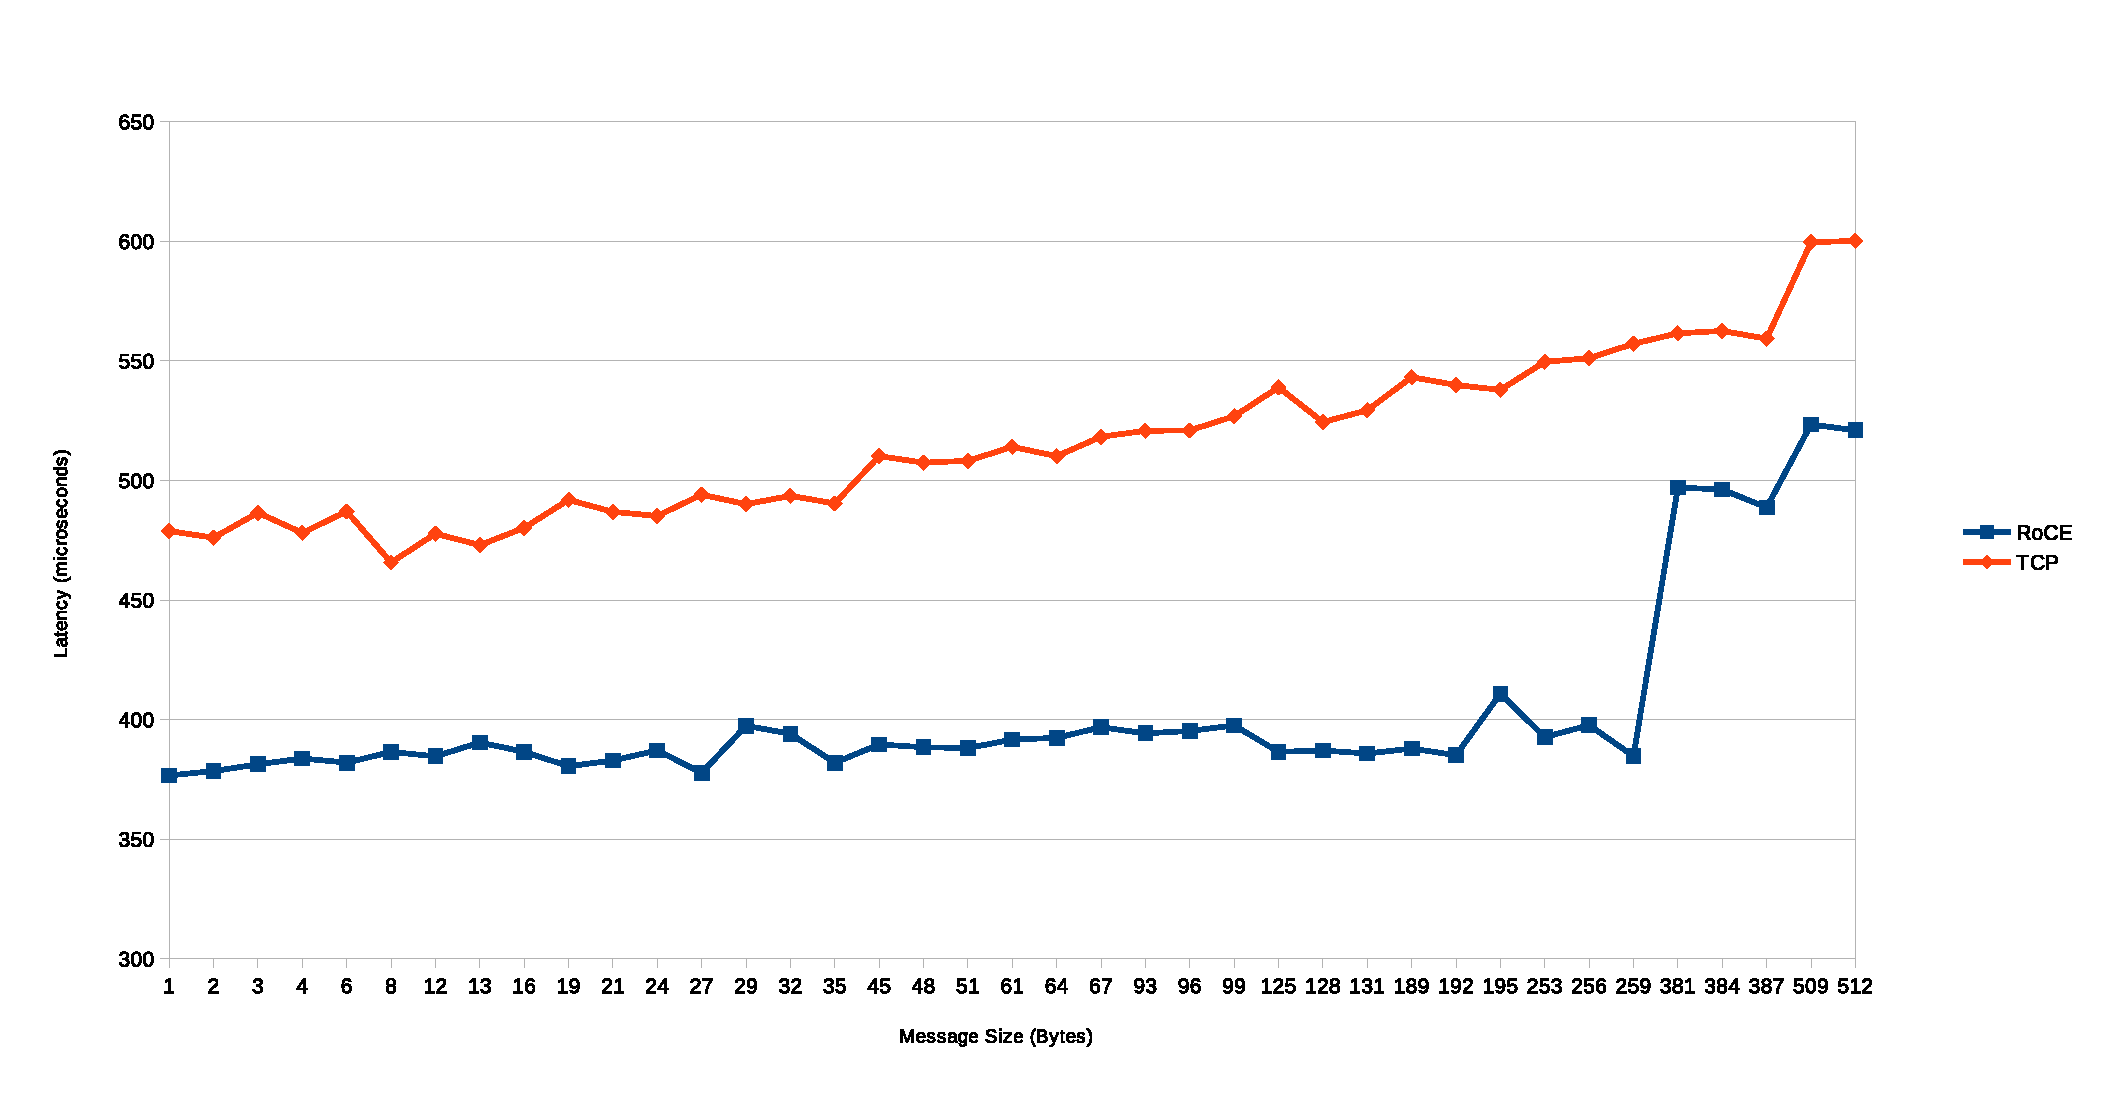
\includegraphics[width=\textwidth]{netpipe_lat_small}
\caption{NetPIPE MPI Latency Results, Small Message Sizes}
\label{npmpi-llat}
\end{figure}

The trend of performance improvement with RoCE continues until message size
rises above 8 KB, after which RoCE latency is significantly higher than TCP
latency. %% This was actually really surprising. Can't explain it...yet

\begin{figure}[H]
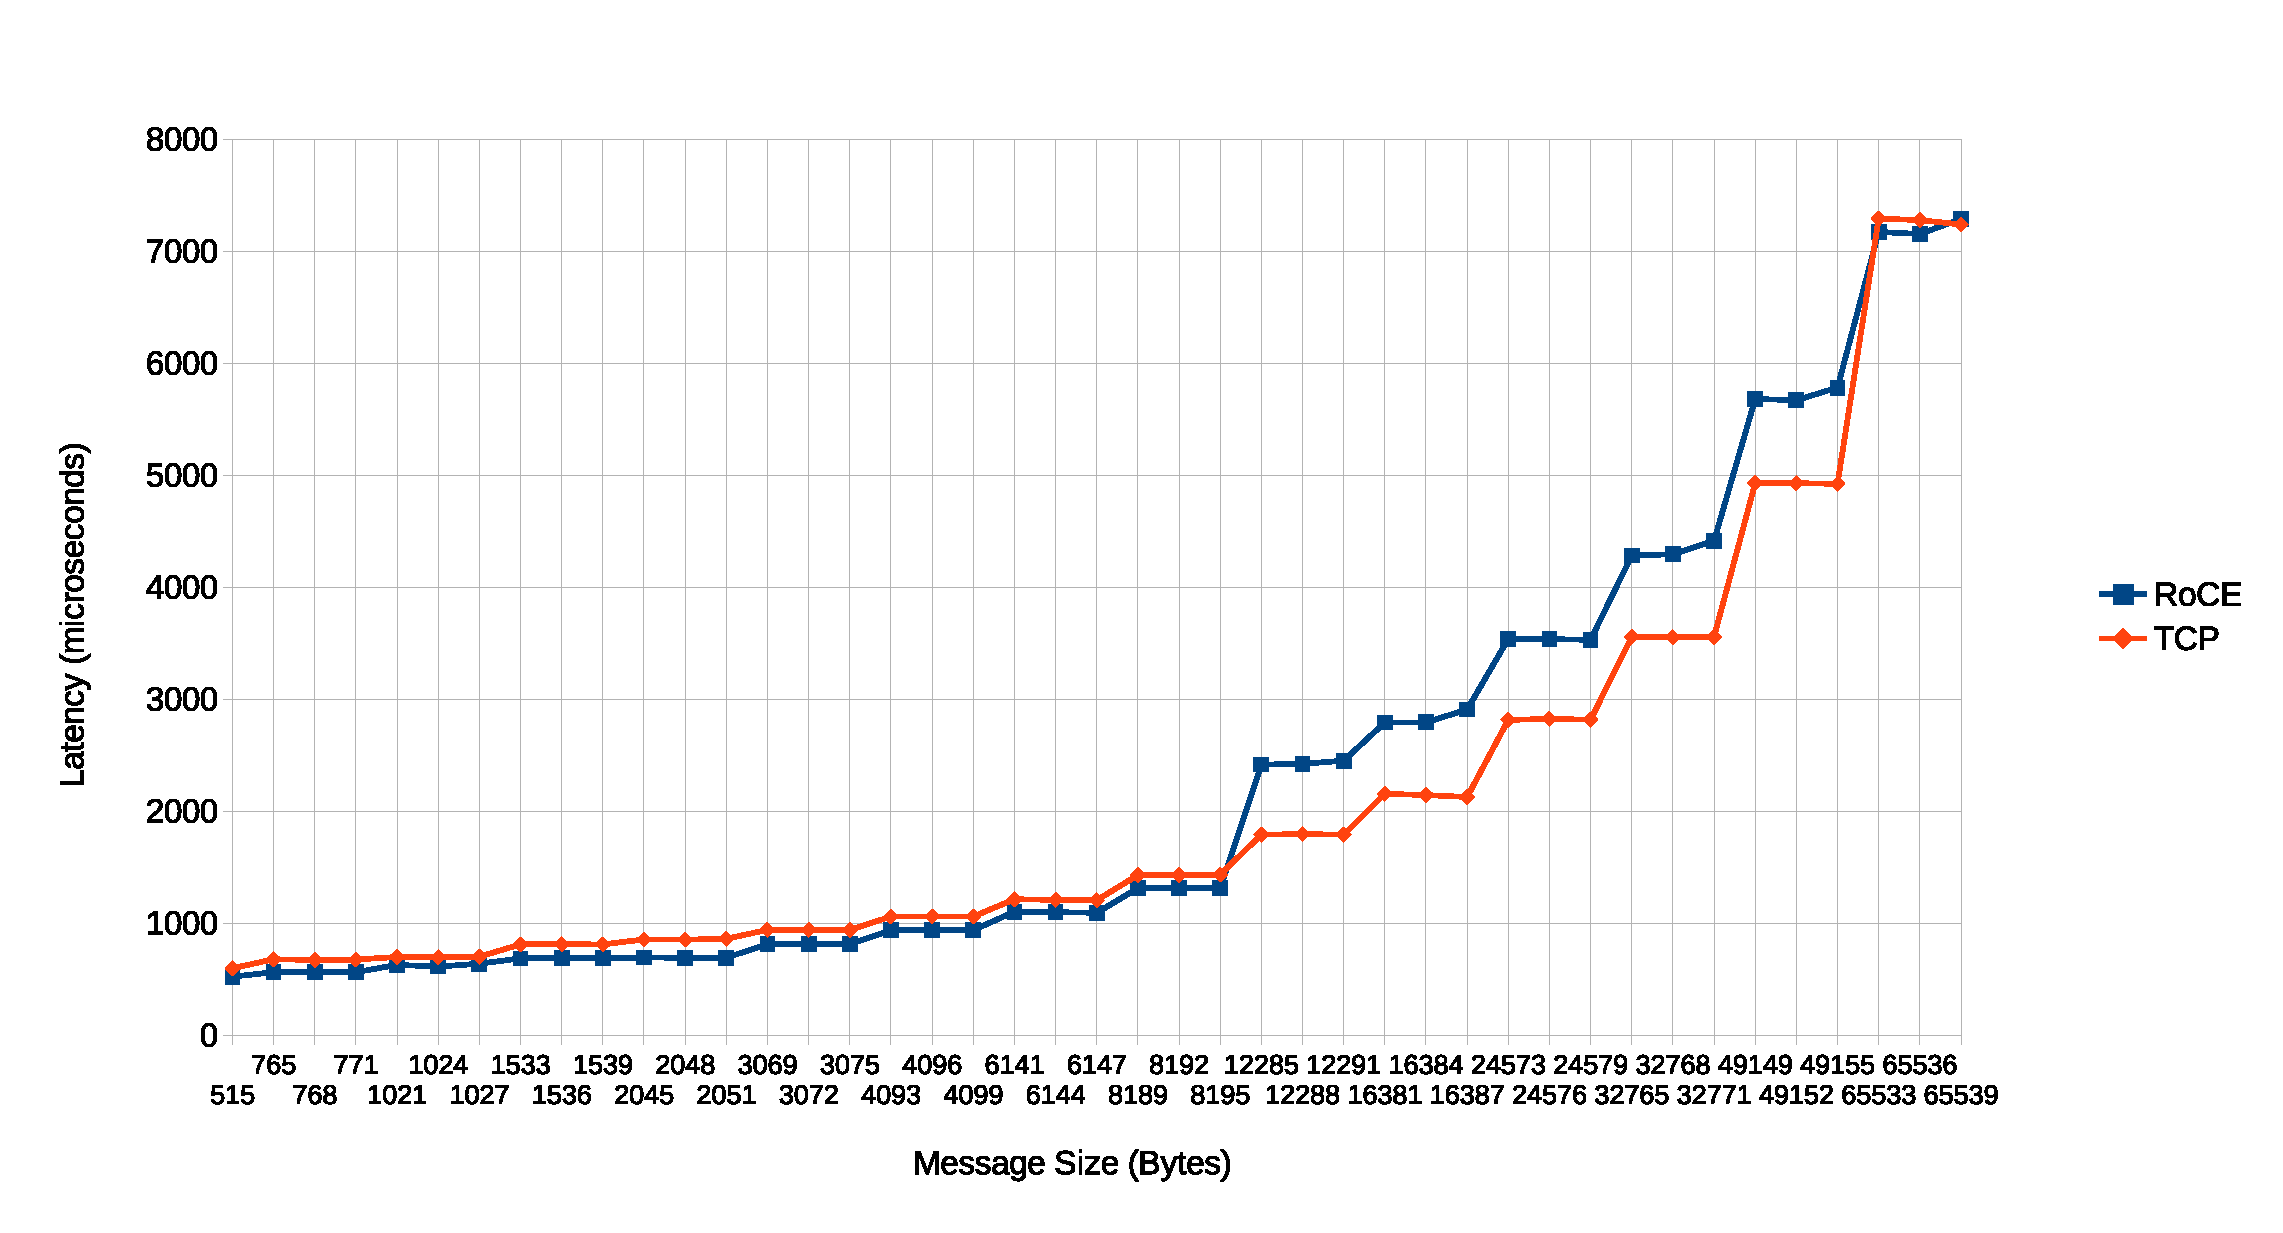
\includegraphics[width=\textwidth]{netpipe_lat_large}
\caption{NetPIPE MPI Latency Results, Large Message Sizes}
\label{npmpi-hlat}
\end{figure}

The MPI bandwidth results in Figures \ref{npmpi-lbw} and \ref{npmpi-hbw} mirror
the latency results. Interestingly, neither TCP nor RoCE traffic could saturate
the 100 Mbps link. %% Is this because the processor can't move data around
%% fast enough? If so, this could have implications on the discussion of GbE
%% modules for the XU. We could also blame the NIC, Linux, or even NetPIPE. I
%% might have to add a way to bypass the rxe flow control...

\begin{figure}[H]
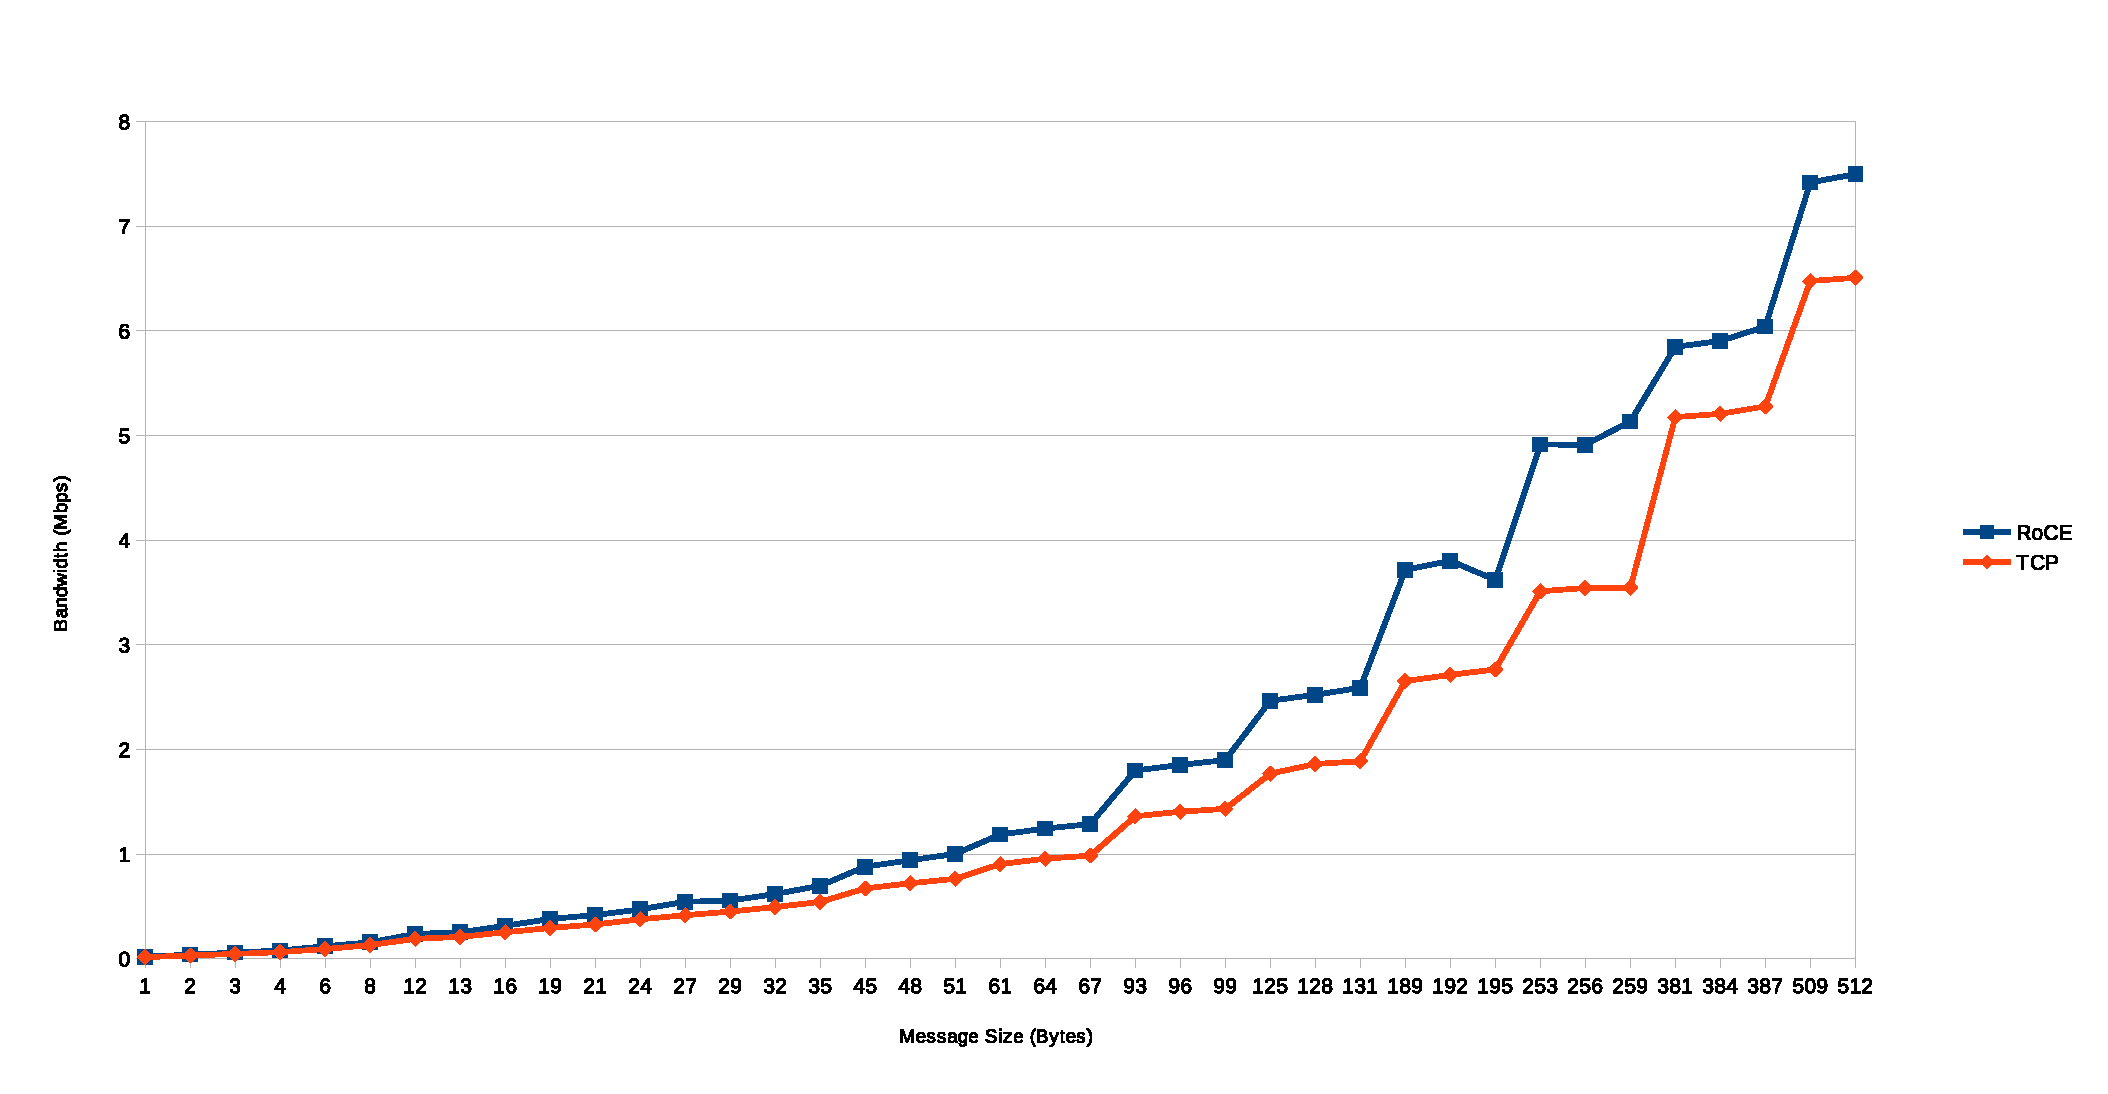
\includegraphics[width=\textwidth]{netpipe_bw_small}
\caption{NetPIPE MPI Bandwidth Results, Small Message Sizes}
\label{npmpi-lbw}
\end{figure}



\begin{figure}[H]
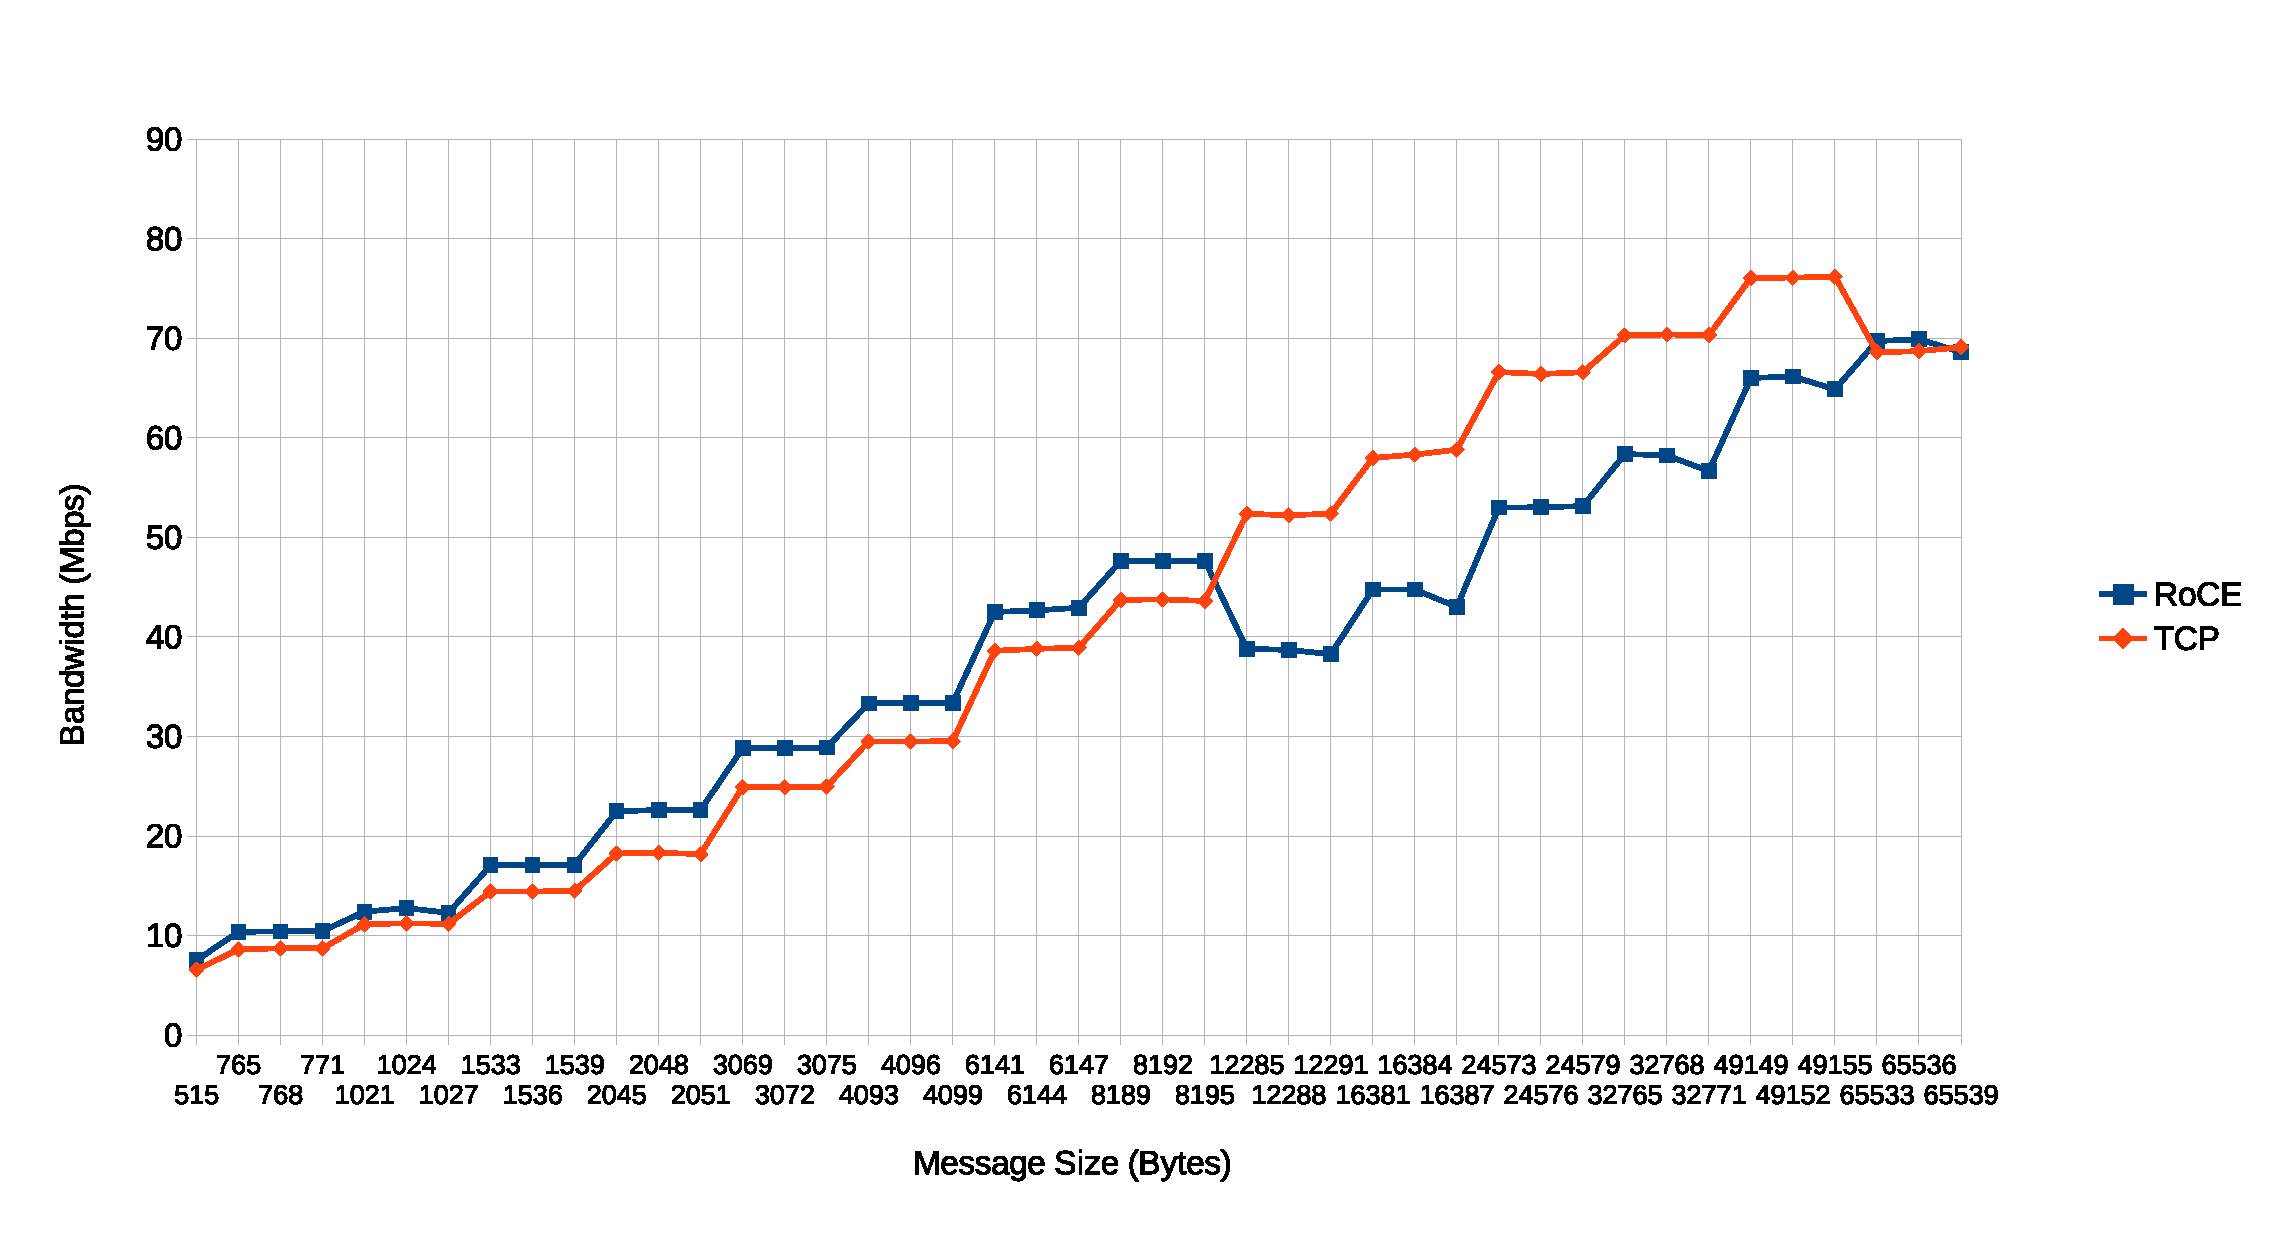
\includegraphics[width=\textwidth]{netpipe_bw_large}
\caption{NetPIPE MPI Bandwidth Results, Large Message Sizes}
\label{npmpi-hbw}
\end{figure}

In order to test transport scalability over MPI in the ODROID platform, we used
the Intel MPI Benchmarks (IMB) suite's ``MultiPingPong'' test with four, six,
and eight MPI processes. This benchmark creates pairs of processes that perform
a standard ping-pong test in parallel with the other pairs. We suspected that
the reduced CPU requirements of the IB transport would lead to slower scaling of
latency as network and I/O bus congestion increases. Figure \ref{multipingpong}
supports this conjecture. In fact, the rxe driver appears to thrive in a
congested networking environment, while TCP/IP latency grows steadily. It
appears that the increased network activity may be hiding some of the latency
introduced by the Ethernet adaptor. %% How?

\begin{figure}[H]
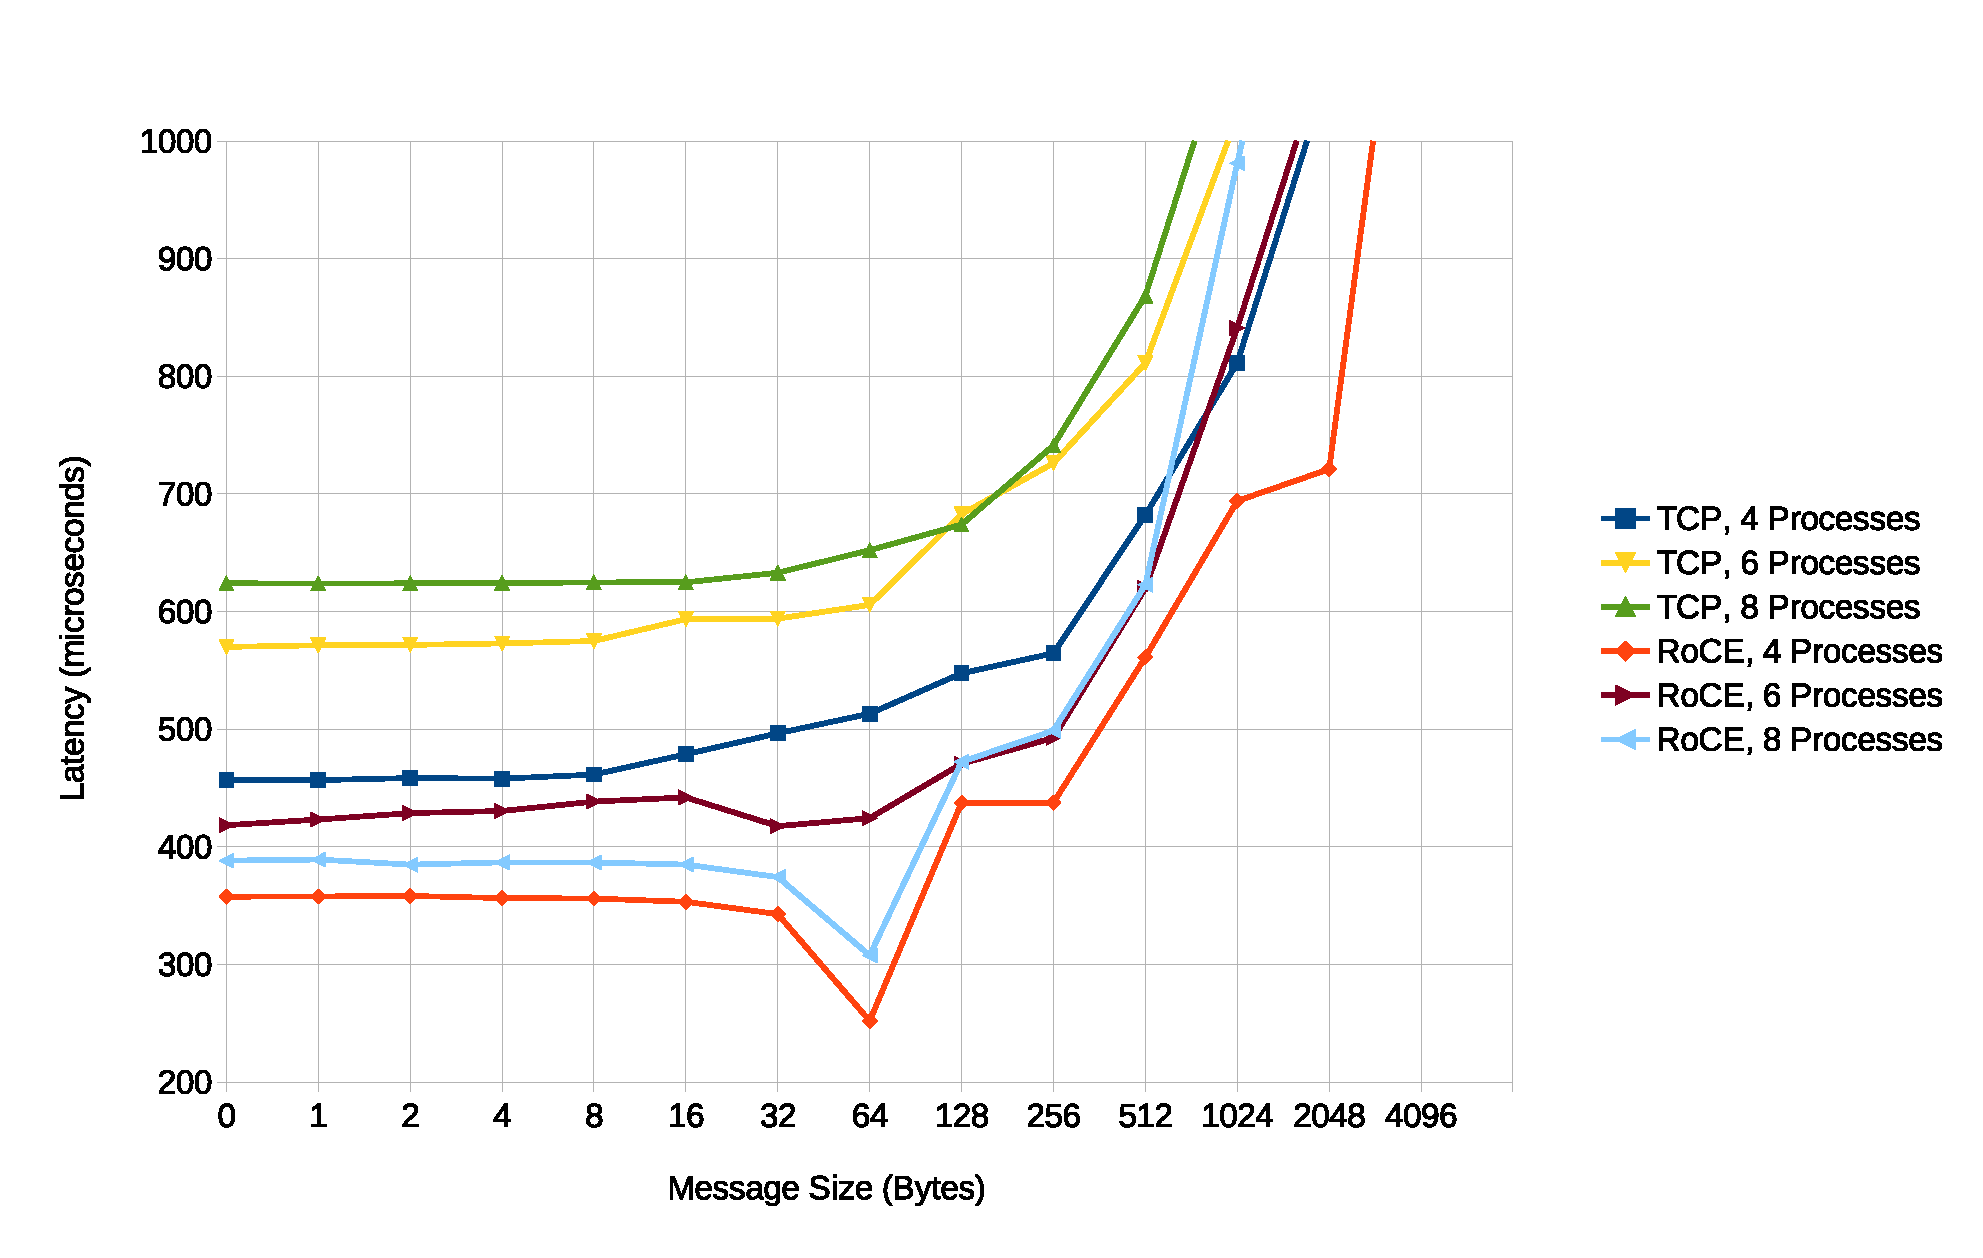
\includegraphics[width=\textwidth]{pingpong_multi_zoom}
\caption{Scaling of Message Latency with Link Congestion}
\label{multipingpong}
\end{figure}

\subsubsection{\textbf{Four ODROID-XU nodes}}

\newpage
\section{\textbf{Conclusions}}
\label{conclusions}

\bibliographystyle{abbrv}
\bibliography{refs}

\end{document}
